\section{Implementation}
\begin{frame}{Ideen}
placeholder
\end{frame}

\begin{frame} {Kommunikation \& Gewinner Berechnung}

\end{frame}

\begin{frame}{Parallelisierungsschema}
	\begin{picture}(0,0)
		\put(30,-80){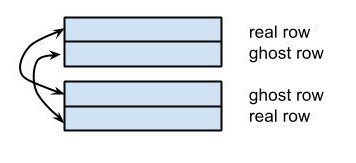
\includegraphics[scale=0.90]{finalPresentation/pics/real-ghost-rows.jpg}}
	\end{picture}
\end{frame}

\begin{frame}{Parallelisierungsschema}
	\begin{picture}(0,230)
		\put(-120,0){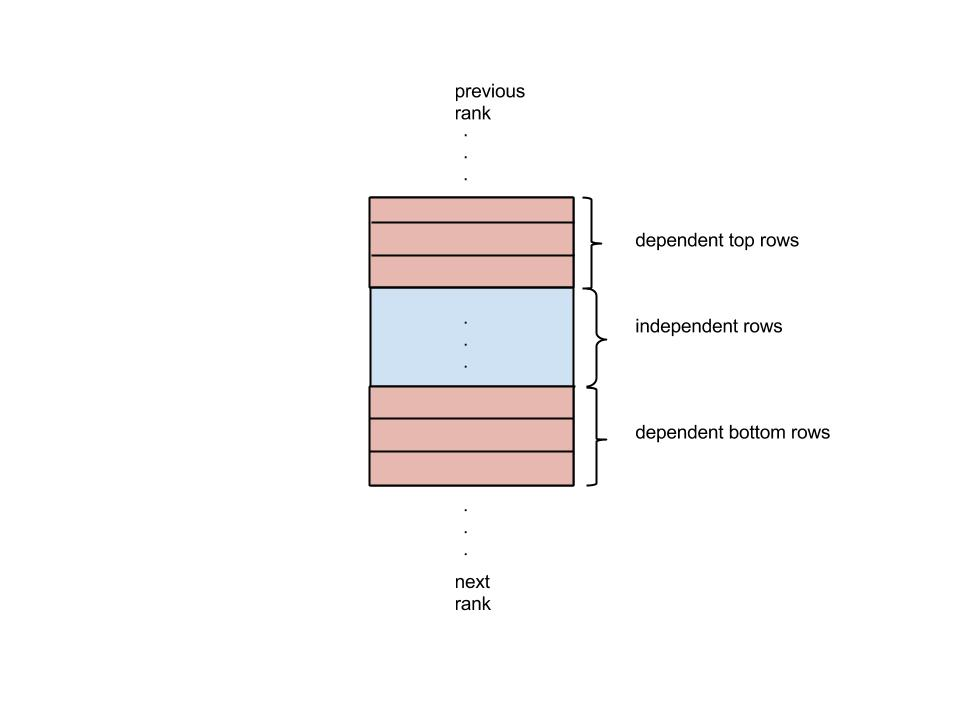
\includegraphics[height=8cm]{finalPresentation/pics/dependent-rows.jpg}}
		\put(170,180){\begin{minipage}[t]{0.4\linewidth}{
			\begin{itemize}
				\item[1] Bewegung der independent ideas
				\item[2] Bewegung der top dependent ideas, Kommunikation dieser
				\item[3] Bewegung der bottom dependent ideas, Kommunikation dieser
			\end{itemize}
			}
		\end{minipage}}
	\end{picture}
\end{frame}

\begin{frame}[fragile]{Parallelisierungsschema}
\begin{lstlisting}[language=C,basicstyle=\small,keywordstyle=\color{black}]
#define send_ideas(ideas_arr, to, tag, req) 
  MPI_Isend(ideas_arr, num_cols, 
    mpi_idea_type, to, tag, MPI_COMM_WORLD, &req) 

#define receive_ideas_into(ideas_arr, from, tag, req) 
  MPI_Irecv(ideas_arr, num_cols, 
    mpi_idea_type, from, tag, MPI_COMM_WORLD, &req) 
\end{lstlisting}
\end{frame}

\begin{frame}[fragile]{Parallelisierungsschema}
\begin{lstlisting}[language=C,basicstyle=\small,breaklines=true,keywordstyle=\color{black}]
#define mpi_define_idea_type()                                               
  int blocklengths[5] = {1,1,1,1,1};                                  
  MPI_Datatype types[5] = {MPI_INT,MPI_INT,MPI_INT, MPI_INT, MPI_INT};       
  MPI_Datatype mpi_idea_type;                                                
  MPI_Aint offsets[5];                                                   
  offsets[0] = offsetof(Idea, a);                                            
  offsets[1] = offsetof(Idea, b);                                            
  offsets[2] = offsetof(Idea, c);                                            
  offsets[3] = offsetof(Idea, h);                                            
  offsets[4] = offsetof(Idea, empty);                                        
    MPI_Type_create_struct(5, blocklengths, offsets, types, &mpi_idea_type); 
    MPI_Type_commit(&mpi_idea_type);                                         
\end{lstlisting}
\end{frame}
